\documentclass{article}

\usepackage{epsfig,graphics,psfrag,color,rotating}
\usepackage{amsmath,amsfonts,amssymb,bbm}


\textwidth=30cm

\def\X{\mathcal{X}}
\def\un{\mathbbm{1}}

\sloppy


\begin{document}
\thispagestyle{empty}

\begin{figure}
%
\centerline{ 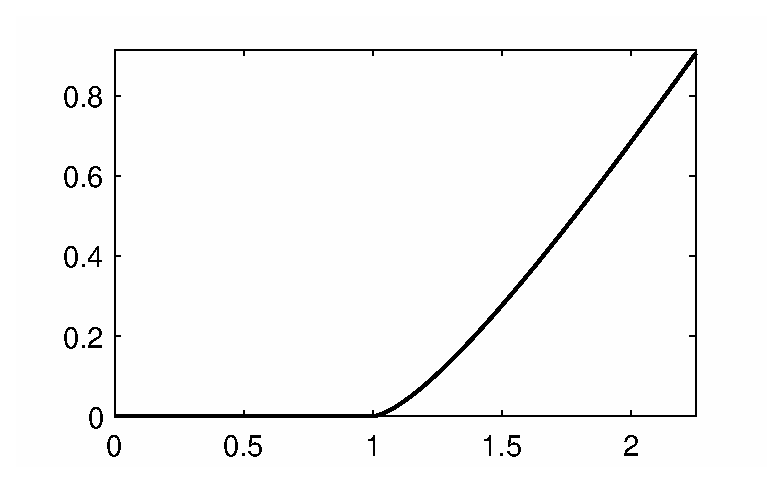
\includegraphics[width=6.5cm]{../EPS/Arcsine_moy}}
\begin{picture}(0,0)
\put(430,6.5){\footnotesize $u$}
\put(334.75,62){\footnotesize \rotatebox{90}{$\phi_{\mathrm{u}}$}}
\put(364,104){\footnotesize $T_{\pm,1}(x) = x \un_{\X_\pm}(x)$}
\end{picture}
\end{figure}

\end{document}
